\documentclass[11pt,a4paper,leqno]{article}
\usepackage{a4wide}
\usepackage[T1]{fontenc}
\usepackage[utf8]{inputenc}
\usepackage{float, afterpage, rotating, graphicx}
\usepackage{longtable, booktabs, tabularx, multirow}
\usepackage{verbatim}
\usepackage{eurosym, calc, chngcntr}
\usepackage{amsmath, amssymb, amsfonts, amsthm, bm, delarray}
\usepackage{caption}
\usepackage{tkz-graph}
\usetikzlibrary{arrows,positioning,snakes,shapes,shapes.multipart,patterns,mindmap,shadows}

\usepackage[toc,page]{appendix} %%Umgebung für Appendix

\numberwithin{equation}{section} %Nummerierung der Gleichungen entspr. Section


\usepackage{bbm} %indicator fct

%referencing
%\usepackage[natbibapa]{apacite}
\usepackage[
    natbib=true,
    bibencoding=inputenc,
    bibstyle=authoryear-ibid,
    style=bwl-FU,
    %citestyle=authoryear-comp,
    maxcitenames=3,
    maxbibnames=10,
    useprefix=false,
    sortcites=true,
    backend=biber
      ]
   {biblatex}
\AtBeginDocument{\toggletrue{blx@useprefix}}
\AtBeginBibliography{\togglefalse{blx@useprefix}}

  \addbibresource{Bibliography/MetricsBibliography.bib}
 \usepackage[unicode=true]{hyperref}
 \renewcommand{\theenumi}{\roman{enumi}}
 \hypersetup{colorlinks=true, linkcolor=black, anchorcolor=black, citecolor=black, filecolor=black, menucolor=black, runcolor=black, urlcolor=black}
 \setlength{\parskip}{.5ex}
 \setlength{\parindent}{0ex}
 
 %Packages David
 \usepackage{comment}
 \usepackage{tikz}
 \usepackage{subcaption}
 
 %Packages Tobi
 
 \usepackage{algorithm}
 \usepackage{algpseudocode}

 %Seitenlayout
 \usepackage{geometry}
 \geometry{a4paper,
 left=3cm,
 right=2cm,
 top=2cm,
 bottom=2cm}
 \usepackage[onehalfspacing]{setspace}

%\theoremstyle{definition}
%!TeX spellcheck = en-US,en-DE

%Umgebung für Theoreme, Propositionen, Lemma
\theoremstyle{definition}
\newtheorem{definition}{Definition}[section]
\newtheorem{proposition}{Proposition}[section]
\newtheorem{corollary}{Corollary}[section]
\newtheorem{theorem}{Theorem}[section]
\newtheorem{assumption}{Assumption}
\newtheorem*{remark}{Remark}
\newtheorem*{claim}{Claim}

\begin{document}
\pagenumbering{gobble}

\begin{titlepage}
	\centering
	{\scshape\LARGE University of Bonn \par}
	\vspace{1cm}
	{\scshape\Large Term Paper in the Project Module Econometrics and Statistics WS 17/18\par}
	\vspace{1.5cm}
	{\huge\bfseries Bagging Regression Trees\par}
	\vspace{2cm}
	{\Large\itshape Robin Kraft, Tobias Felix Werner and David Zeimentz\par}
	\vfill
	supervised by\par
	Professor~Alois \textsc{Kneip} \par
	JProfessor~Dominik \textsc{Liebl}
	\vfill

% Bottom of the page
	{\large \today\par}
\end{titlepage}
\newpage

\pagenumbering{roman} %Seitenzahlen Römisch
\tableofcontents
\newpage

%List of Figures
\listoffigures
\addcontentsline{toc}{section}{List of Figures}

%List of Tables
\listoftables
\addcontentsline{toc}{section}{List of Tables}

\newpage

%%%%%%%%%%%%% H A U P T T E I L %%%%%%%%%%%%%%%%
\pagenumbering{arabic} %Seitenzahlen ab hier arabisch

%Intro
\section{Introduction}
In statistical estimation, most prediction problems encounter a bias-variance tradeoff. \\
A class of predictors for which this is pronounced are so-called Regression Trees (\cite{Breiman1984}). 
Those kind of predictors partition the domain of the explanatory variables by a recursive algorithm and fit then a simple regression model to each resulting region. 
While yielding low biased estimates due to flexible adaption to the data, Tree predictors react very sensitive to small changes in the underlying dataset.
This high variance caused by the recursive structure of the algorithm can
result in large changes in the predicted values. \cite{breiman1996B} declares such kind of predictors as unstable.\\
The so-called Bagging algorithm proposed by \cite{Breiman1996} bypasses this tradeoff by reducing the variance of the unstable predictor, while leaving its bias mostly unaffected.
In particular, Bagging uses repeated bootstrap sampling to construct multiple versions of the same prediction model like Regression Trees and averages over the resulting predictions.\\
In this paper we will show that Bagging can reduce the variance of Regression Tree predictors and thereby improves their prediction accuracy in terms of the mean squared prediction error (MSPE).\\
For this, we illustrate the theoretical framework given in \cite{Buhlmann2002} tailored to Regression Trees. In particular, they show that Bagging smooths discontinuities induced by the Regression Tree predictor which leads to a variance reduction.
Focusing on the simplest type of Regression Trees, so-called Stump predictors, their theoretical treatments of Bagging however has its limitations due to the non-normal distribution of the predictor and therefore the failure of the bootstrap. When replacing the bootstrap procedure of Bagging by subsampling without replacement, they obtain a method that is more traceable from a theoretical perspective under very mild assumptions. Using this method, called Subagging, it is possible to state upper bounds for the variance and mean squared error of the predictor given an appropriate choice of the subsample size.\\
Our simulation studies and application to a real data set undermine the presented theoretical framework and are in line with former findings (e.g. \cite{breiman1998}, \cite{Bauer1999} and \cite{Dietterich2000}). Bagging can achieve a reduction of the MSPE of up to  50\% compared to unbagged Regression Trees. 
A critical point in order to calculate the bagged predictor are the number of bootstrap iterations. 
Our simulation studies suggest that 50 bootstrap replications are sufficient.\\ 
It is common practice to restrict the model complexity of the Tree predictor in order to govern the bias variance tradeoff. However, our simulation results indicate that the higher the model complexity the greater the MSPE-reduction via Bagging will be.\\
While Subagging is more traceable from a theoretical perspective, our simulations suggest that Subagging with half of the dataset can achieve approximately the same results as Bagging.\\
In the literature it is widely discussed why Bagging works. \\
\cite{Grandvalet2004} argues that Bagging lessens the importance of observations which have a high influence on the prediction accuracy.
He concludes that depending on whether the observation would improve the prediction performance or not, Bagging can be beneficial or harmful.\\
Another theoretical framework based on continuous and differentiable predictors is provided by \cite{friedman2007}.
Their argument relies on a decomposition of the predictor into a linear and non-linear component via a truncated Taylor series.
Based on a heuristic argument, they conclude that Bagging reduces the variance of the non-linear part while leaving the linear component unaffected.\\
For the concept of generalized averages (U-statistics) \cite{buja2006} show that Bagging can increase both bias and variance.
Furthermore, they show that Subagging with half of the data set is equivalent to Bagging in this case.
For Tree predictors they observe empirically that this kind of Subagging yields approximately the same results as Bagging.\\
The rest of this paper is structured as follows.
Section 2 introduces Regression Trees as an example for an unstable predictor. Section 3 and 4 analyze Bagging and Subagging and relates them to Regression Trees.
In Section 5 simulation results are presented. Section 6 applies Bagging and Regression Trees to a real world data set.
A summary and concluding remarks can be found in section 7. Proofs are collected in the Technical Appendix \ref{sec:Tec_App}.



%Trees

\section{Regression Trees}
The predictors which are most frequently used in combination with Bagging are Classification and Regression Trees. We focus on Regression Trees, which are used to predict a numerical response variable.\footnote{Although tree-based methods are most frequently used for classification problems we want to restrict our attention to Regression Trees. In classification settings problems arise which are not essential to the analysis of Bagging. An example is the proper choice of accuracy  measure. In a regression setup, the residual sum of squares is used, but this measure is not suitable for classification. Here the best choice of measure is not clear.} Although Regression Trees exhibit a low bias, they are not competitive to other prediction methods as they react sensitive to changes in the data and therefore have a large variance. In combination with Bagging and its variance reducing effect bagged Regression Trees provide a powerful tool for prediction. The formal presentation of Regression Trees follows \cite{EoSL}. For a detailed treatment of Regression Trees implemented with the CART algorithm see \cite{Breiman1984}.

\noindent
\subsection{Prediction using Regression Trees}\label{sec:Tree_Pred}
Consider the following setting. Assume we are interested in the prediction of a continuous response variable denoted as $y$ on the basis of a set of $p$ explanatory variables $\mathbf{x}=(x_1,x_2,...,x_p)^T$. Furthermore, assume our data consists of $n$ observations, so we have $L_i = (y_i,\mathbf{x}_i)$ for data instances $i=1,...,n$. The setting and denotations carry over to subsequent sections.\\
A Regression Tree model consists of a sequence of binary decision rules, which can be summarized in a tree diagram. A decision rule is defined by an explanatory variable (splitting variable) and a value in the domain of the respective variable (split point). We refer to decision rules as nodes. An exemplary Regression Tree for a two-dimensional predictor space $\mathbf{x}=(x_1,x_2)^T \in [0,1]^2$ is provided in Figure \ref{fig:Tree_FigTreePar} (a).

\begin{figure}[htb]
\centering
\begin{minipage}[c]{.45\linewidth}
\centering
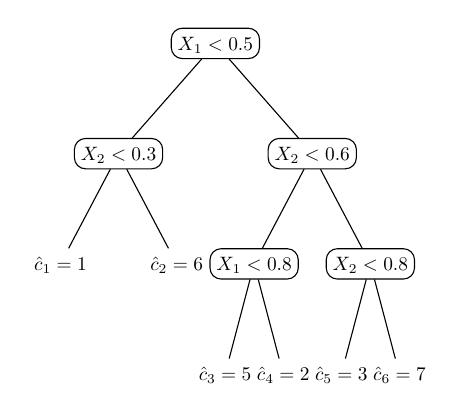
\begin{tikzpicture}[
scale = 0.7,
every node/.style={transform shape},
baseline,
level distance=20mm,
text depth=.1em,
text height=.8em,
level 1/.style={sibling distance=10em},
level 2/.style={sibling distance=6em},
level 3/.style={sibling distance=3em}]


	\node [rounded corners, draw] {$X_1 < 0.5$}
		child {node [rounded corners, draw] {$X_2 < 0.3$}
			child {node {$\hat{c}_1=1$}}
			child {node {$\hat{c}_2=6$}}
		}
		child {node [rounded corners, draw] {$X_2 < 0.6$}
			child {node [rounded corners, draw] {$X_1<0.8$}
				child {node {$\hat{c}_3=5$}}
				child {node {$\hat{c}_4=2$}}
			}
			child {node [rounded corners, draw] {$X_2<0.8$}
				child {node {$\hat{c}_5=3$}}
				child {node {$\hat{c}_6=7$}}
			}
	};

\end{tikzpicture}
\subcaption{Illustration Regression Tree}
\end{minipage}%
\hfill%
\begin{minipage}[c]{.45\linewidth}
\centering
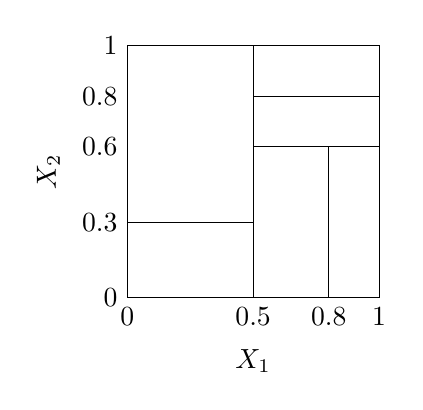
\begin{tikzpicture}[scale = 0.8]

\draw (0,0) -- (4,0) -- (4,4) -- (0,4) -- (0,0);
\draw (2,0) -- (2,4);
\draw (0,1.2) -- (2,1.2);
\draw (2,2.4) -- (4,2.4);
\draw (2,3.2) -- (4,3.2);
\draw (3.2,0) -- (3.2,2.4);
\node [left] at (0,0) {0};
\node [left] at (0,1.2) {0.3};
\node [left] at (0,2.4) {0.6};
\node [left] at (0,3.2) {0.8};
\node [left] at (0,4) {1};
\node [below] at (2,0) {0.5};
\node [below] at (0,0) {0};
\node [below] at (4,0) {1};
\node [below] at (3.2,0) {0.8};
\node[rotate=90] at (-1.25,2) {$X_2$};
\node at (2,-1) {$X_1$};
\end{tikzpicture}
\subcaption{Illustration Partition}
\end{minipage}
\caption[Illustration of a Regression Tree and its corresponding Partition]{Illustration of a Regression Tree and its corresponding Partition}
\label{fig:Tree_FigTreePar}

\end{figure}


\noindent
A prediction for a new observation $\mathbf{x^{new}}$ is obtained by following down the tree diagram, starting at the top node. At each node continue on the left branch if the decision rule is satisfied and on the right if not. This procedure is continued until a final branch of the tree diagram is reached. We refer to final branches as terminal nodes and to the number of final branches as size of the Tree. Each terminal node is labeled with a constant $\hat{c}_k$ with $k \in \{1,...,6\}$. This constant is used as predicted value for an observation $\mathbf{x^{new}}$ reaching the corresponding terminal node. For instance, the prediction for an exemplary observation $\mathbf{x^{new}}=(0.4,0.4)^T$ using the Regression Tree of Figure~\ref{fig:Tree_FigTreePar}~(a) is $\hat{c}_2=6$.

\subsection{The CART Algorithm}
The method which is most widely used to construct Regression Trees is the so-called Classification and Regression Tree (CART) algorithm developed by \cite{Breiman1984}. The basic idea of the procedure is to group data with similar characteristics. For this, the CART algorithm partitions the feature space (spanned by $x_1, ..., x_p$) by successive binary splits. These binary splits correspond to the decision rules of the tree diagram. Each terminal node corresponds to a region in the partition and the corresponding constant is used as predicted value for an observation falling into the respective region. A graphical illustration of the two-dimensional example is provided in Figure \ref{fig:Tree_FigTreePar} (b).

Repeated binary splits are a reasonable simplification as the determination of the best binary partition is computational infeasible\footnote{The best binary partition would require to calculate for any sequence of binary splits and any possible split point at each node the residual sum of squares of the resulting predictor, which is computationally infeasible.} (see Hyafil and Rivest (1976)). The CART algorithm is computational feasible, as the determination of the split point can be done quickly and the procedure has to be repeated for only $p$ input variables (Hastie et al. (2009, p.307)). However, this procedure might not result in the best binary partition.\\


\noindent
The CART algorithm works as follows. In the first step, the entire feature space is split at split point $d$, using splitting variable $x_j$ ($j \in \{1,...,p\}$), into two regions denoted as $R_1$ and $R_2$. Equivalently we can think of dividing the entire data set into two subsets. These regions are defined as
$$R_1(j,d)=\{\mathbf{x}|x_j \le d\} \text{ and } R_2(j,d)=\{\mathbf{x}|x_j > d\}.$$
\noindent
Split point $d$ and splitting variable $x_j$ are chosen such that the residual sum of squares is minimized in the resulting regions. This means $d$ and $x_j$ are chosen such that following minimization problem is solved.
\begin{equation}
\label{eq:CARTmin}
\min\limits_{j,d}[\min\limits_{c_1}\sum\limits_{\mathbf{x_i} \in R_1(j,d)}(y_i-c_1)^2 + \min\limits_{c_2}\sum\limits_{\mathbf{x_i} \in R_2(j,d)}(y_i-c_2)^2]
\end{equation}
\noindent
The inner minimization problem determines the best choice (in terms of residual sum of squares) of the constants in the resulting regions. The best choice is simply the sample average of observations in the respective region (Breiman et al. (1984, p. 230)). The outer minimization problem selects the optimal split point and the optimal splitting variable. To solve this problem we determine for each splitting variable the optimal split point and then select the splitting variable yielding the lowest residual sum of squares. We denote the optimal choice of splitting point by $d^0$ and the optimal constant by $c^0$. Estimates are denoted as $\hat{d}$ and $\hat{c}$, respectively. In the next step the CART algorithm considers the resulting regions and applies the same procedure to them. Therefore the method is known as \textit{binary recursive splitting}.  The procedure is repeated until a stopping rule is satisfied, for instance if a minimum amount of observations in each terminal node is achieved. An alternative stopping rule prescribes to add further nodes as long as the next node reduces residual sum of squares by a predetermined amount.

Now consider a partition of the feature space into $K$ regions $R_1,...,R_K$. The regression function for this partition can be expressed as follows
\begin{equation}
\label{eq:CARTpred}
\hat{\theta}(\mathbf{x})= h_{n}(L_{1},\dots, L_{n})(\mathbf{x})=\sum\limits_{k=1}^{K}\hat{c}_k\mathbbm{1}_{[\mathbf{x}\in R_k]}, 
\end{equation}
where the function  $h_n:\mathbb{R}^{p} \rightarrow \mathbb{R}$ is the CART algorithm.\\
Similarly to the solution to the inner minimization problem of \eqref{eq:CARTmin} the optimal choice for the constant is given by the sample average of observations in the respective region (Breiman et al. (1984, p.230)). Expression \eqref{eq:CARTpred} reveals that the true data generating process is approximated by a piecewise constant step function.

\subsection{Bias-Variance Tradeoff} \label{sec:BiasVariance}
Breiman et al. (1984, p.272) state that any further node will never increase the (expected) sum of squared errors. This means that any further split will (weakly) improve the fit to the initial data set. For instance, if we grow a Tree to its maximal size, i.e. until only one observation is left in each terminal node, the initial data set is fit identically. The number of terminal nodes is governed by stopping rules. Consequently, stopping rules influence the flexibility of the regression function to adapt to the data set. 

First consider a stopping rule which allows for large Regression Trees. These models can adapt flexibly to any complex true relationship in the data and will therefore exhibit a low bias. The problem with this adaptiveness is the risk of fitting the artificial noise in the data (overfitting). Fitting the artificial noise of the data will result in a sensitivity to changes in the data, i.e. a high variance. In contrast, if we select a more restrictive stopping rule we might not capture the fundamental relationships in the data (underfitting). However, this procedure will be more robust to changes in the data. In conclusion we encounter a tradeoff between bias and variance in the specification of Regression Tree models, which is governed by stopping rules.\footnote{This trade-off between bias and variance is not specific to Regression Trees but rather a common problem in statistical modeling.}

\subsection{Instability}\label{sec:stability}
Regression Trees react particularly sensitive to changes in the data. Consider a small perturbation of the initial data set and assume this small perturbation already leads to a change of the split point or splitting variable at a top node. Due to the recursive structure all decisions followed by this node are affected as well. Therefore the change in the data will have a large impact on the resulting predictor (Breiman et al. (1984, p.156-159)). A graphical illustration of the instability of Regression Trees is provided in Appendix \ref{sec:instability}. \cite{Breiman1996} denote predictors for which a small perturbation in the data set leads to significant changes in the predictor as instable. The instability of Regression Trees is pointed out by \cite{breiman1996B}. For the theoretical analysis of Bagging a formal definition of the notion of instability is required. \cite{Buhlmann2002} provide the following definition which is not inconsistent with the heuristic definition by \cite{breiman1996B}.

\begin{definition}[Stability of a predictor] \label{stability}
A statistic $\hat{\theta}_{n}(\mathbf{x}) = h_{n}(L_{1},\dots, L_{n})(\mathbf{x})$ is called stable at $\mathbf{x}$ if $\hat{\theta}_{n}(\mathbf{x}) = \theta(\mathbf{x}) + o_{p}(1) \: (n \rightarrow \infty)$ for some fixed value $\theta(\mathbf{x})$.
\end{definition}

\noindent
This definition resembles the definition of consistency. The crucial difference is that the statistic $\hat{\theta}_n(\mathbf{x})$ does not need to converge to the true population parameter, but only to a stable limit $\theta$. This means that an unstable predictor will assume a different limit value for another data set (taken from the same data generating process) with positive probability, even if the size of the data set goes to infinity. 



%Bagging
\section{Bagging}\label{bag}

\subsection{Algorithm}
Bagging (bootstrap aggregation) first proposed by \cite{Breiman1996} can improve the prediction performance of an algorithm or statistical estimator by reducing its variance while not increasing the bias too much (relative to the variance reduction).\\
Bagging is based on the idea that the variance of the sample average is weakly smaller than the variance of the individual random variables.
To make this more precise, let $X_1, \dots, X_n$ be i.i.d. random variables with $\mu = E[X_1]$ and $\sigma^2 = Var[X_1]$.
Let $\bar{X}= \frac{1}{n}\sum_{i=1}^{n}X_{i}$.
Due to independent (first equality) and identically distributed (second equality) random variables, it holds that
$$
Var[\bar{X}]= \frac{1}{n^2} \sum_{i=1}^{n} Var[X_i]=\\
\frac{\sigma^2}{n} \leq \sigma^2.
$$
Observe also that the sample average is unbiased,
$$
E[\bar{X}]= \frac{1}{n} \sum_{i=1}^{n} E[X_i] = \mu.
$$
Averaging over the individual random variables reduces the variance while leaving the bias unaffected.
As it will turn out, for Bagging this simple heuristic holds also but there will be an inherent bias-variance tradeoff.\\
Based on those considerations, \cite{Buhlmann2002} define Bagging as follows:

\begin{definition}\label{bagging}(Bagging)
	\begin{enumerate}
	\item Construct a bootstrap sample $L_{i}^{*} = (y_{i}^{*}, \mathbf{x_{i}^{*}}) \:(i = 1, \dots , n)$ (with replacement) according to the empirical distribution of the pairs $L_{i} = (y_{i}, \mathbf{x_{i}}) \: (i = 1, \dots , n)$ i.i.d.
	\item Compute the bootstrapped predictor $\hat{\theta}_{n}^{*}(\mathbf{x})$ by the plug-in principle; that is, $\hat{\theta}_{n}^{*}(\mathbf{x}) = h_{n}(L_{1}^{*}, \dots, L_{n}^{*})(\mathbf{x})$, where $\hat{\theta}_{n}(\mathbf{x}) = h_{n}(L_{1},\dots, L_{n})(x)$.
	\item The bagged predictor is $\hat{\theta}_{n;B}(\mathbf{x}) = E^{*} [\hat{\theta}_{n}^{*}(\mathbf{x})]$
	\end{enumerate}
\end{definition}

The function $h_n(\cdot)$ is obtained by an algorithm as for example CART and $E^*[\cdot]$ denotes the expectation induced by the bootstrap sampling.\\
Consider now the case where we want to predict for a new realization of a covariate vector, say $\mathbf{x^{new}}$, the bagged predicted value.
In order to do this, we argue along Definition \ref{bagging}. Construct first a bootstrap sample $L_i^*$ by sampling with replacement from the original data $L_i$ $(i=1, \dots, n)$.
In the second step, we compute the bootstrapped predictor by constructing a Regression Tree using the bootstrap sample from the previous step.
Applying now the new realization to the bootstrapped predictor yields a  predicted value, say $\hat{y}^*$.
If we repeat steps one and two $B \in \mathbb{N}$ times, we get $B$ different bootstrapped predictors (or equivalently Regression Trees) and hence $B$ different predicted values for the new realization $\mathbf{x^{new}}$, say $\hat{y}_1^*, \dots, \hat{y}_B^*$.
Note that the Regression Trees constructed with the bootstrap samples can differ from each other in their splitting points or splitting variables.
Averaging over $\hat{y}_1^*, \dots, \hat{y}_B^*$ yields the bagged predicted value.\footnote{A graphical illustration of this procedure can be found in Appendix \ref{App:Ill_Bag}.}
In practice, step three is therefore usually obtained via a Monte Carlo simulation (see also Section \ref{sub:simsetup}).\\
Note that in Definition \ref{bagging} the algorithm is written in terms of population.\\
In order to relate Bagging to the notion of stability (Definition \ref{stability}) introduced in Section \ref{sec:stability}, we claim the following:
\begin{claim}
Bagging reduces the variance of unstable predictors.
\end{claim}
\noindent In order to verify this claim, we give a heuristic argument (see also \cite{Breiman1996}).\\
Consider first a stable predictor (i.e. low variance).
If small changes in the data set lead to small changes in the considered predictor $\hat{\theta}_{n}(\cdot)$ then indeed $\hat{\theta}_{n;B}(\cdot)$ should be close to the original predictor and Bagging should therefore have a negligible variance reducing effect.\\
Conversely, for an unstable predictor (i.e. high variance even in the limit), small changes in the data set should cause large changes in $\hat{\theta}_{n}(\cdot)$.
The bootstrapped predictor should also be very different from the original predictor.
By averaging over those predictors the variance of the resulting predictor should be smaller than that of the original one.

%%%%%%%%%%%%%%%%%%%%%%%%%%%%%%%%%%%%%%%%%%%%%%%%%%%%%%%%%%%%%%%%%%%%%%%%%%
\subsection{Introductory Example}\label{introductionbagging}
We start our analysis of Bagging with an introductory example which is adapted from \cite{Buhlmann2002}. \\
Let $Y_{1}, Y_{2}, \dots, Y_{n}$ be i.i.d random variables with $\mu = E[Y_{1}]$ and $\sigma^{2} = Var[Y_{1}]$. Consider first the unbagged predictor,
\begin{equation}\label{unbagged}
\hat{\theta}_{n}(x) = \mathbbm{1}_{[\bar{Y}_{n} \leq x]},\quad x\in  \mathbb{R},
\end{equation}
where $\bar{Y}_{n} = \frac{1}{n}\sum_{i=1}^{n}Y_{i}.$ \\
The indicator function assumes the value one if $x$ is above the threshold $\bar{Y}_n$ and zero otherwise. The analysis of an indicator function is of particular interest as the Tree predictor consists of a sum of indicator functions.\\
We first check if the predictor stabilizes.
Let $x$ for the sake of the argument be fixed.
By the (weak) law of large numbers observe that $\bar{Y}_{n}\xrightarrow{p} \mu.$
The considered predictor converges to a fixed target $\theta(x)=\mathbbm{1}_{[\mu \leq x]}$ as $n$ increases and hence stabilizes according to Definition \ref{stability}.
As $x$ and $\mu$ are fixed, the indicator function will either always assume the value one or zero as $n$ increases.\\
Figure \ref{plot_finite_sample} demonstrates the stabilization of the predictor measured via the mean squared error.
As the predictor gets more and more accurate (due to the (weak) law of large numbers) the mean squared error decreases to zero.
Moreover, observe that Bagging has asymptotically no effect.\footnote{See Appendix \ref{sec:App_FiniteSample} regarding implementation purposes.}
\begin{figure}[t]
\centering
\includegraphics[scale = 0.4]{../../out/figures/theory_part_simulation/plot_finite_sample.pdf}
\caption[Mean squared error for the predictor in (\ref{unbagged}) and a bagged version as a function of $c$ and for sample sizes $n \in \{100, 1000, 10000, 50000\}$ (with $\mu=0$, $\sigma =2$).]{Mean squared error for the predictor in (\ref{unbagged}) and a bagged version as a function of $c$ and for sample sizes $n \in \{100, 1000, 10000, 50000\}$ (with $\mu=0$, $\sigma =2$).}\label{plot_finite_sample}
\end{figure}
However, to analyze the effect of Bagging we require a locally unstable predictor.
For this, we consider a $n^{-1/2}$-neighbourhood around $\mu$
\begin{equation}\label{12region}
 x = x_{n}(c)= \mu + c\sigma n^{-1/2}.
\end{equation}
Note that the second term in this expression is the deviation from the population mean $\mu$ which is governed by the deterministic value $c$.
This choice is dynamic in the sense that as $n$ increases the sequence $x_1(c), x_2(c), \dots$ converges to $\mu$ at the rate $n^{-1/2}$.\\
Note further that by a central limit theorem for $\bar{Y}_{n}$
\begin{equation}\label{clt}
n^{1/2}(\bar{Y}_{n} - \mu ) \xrightarrow{D} \mathcal{N}(0,\,\sigma^{2}).
\end{equation}

Plugging (\ref{12region}) into (\ref{unbagged}) and applying (\ref{clt}), one yields (see proof of the below Proposition \ref{prop1})
$$\hat{\theta}_{n}(x_n(c))=\mathbbm{1}_{[n^{1/2}\frac{(\bar{Y}_{n} - \mu )}{\sigma} \leq c]} \xrightarrow{D} \mathbbm{1}_{[Z \leq c]}, \quad
Z \sim \mathcal{N}(0,1).$$

\begin{remark}
For $n \rightarrow \infty$, it is $not$ the case that $\mathbbm{1}_{[\bar{Y}_{n} \leq x_n(c)]} \rightarrow \mathbbm{1}_{[\mu \leq \mu]}=1$.
In order to see this, observe that (\ref{12region}) converges with the same rate to $\mu$ as $\bar{Y}_n$, namely $n^{-1/2}$.
Intuitively speaking, this means that (\ref{12region}) and $\bar{Y}_n$ will disperse even asymptotically at the same magnitude.
The considered predictor will therefore remain unstable even as $n$ tends to infinity.
\end{remark}

To derive the first and second moments note that the above expression is a Bernoulli-variable and hence
$$E[\hat{\theta}_{n}(x)] \rightarrow P[Z \leq c] = \Phi(c)\quad (n \rightarrow \infty)$$
$$Var[\hat{\theta}_{n}(x)] \rightarrow \Phi(c)(1-\Phi(c)) \quad(n \rightarrow \infty)$$

We have constructed a predictor that is unstable according to Definition \ref{stability} as the variance does not decrease to zero (even as $n \rightarrow \infty$).\\
Consider now a bagged predictor as in Definition \ref{bagging}. Some calculations show that
\begin{equation}\label{bagged}
\begin{split}
\hat{\theta}_{n;B}(x_{n}(c))=E^{*}[\mathbbm{1}_{[\bar{Y}_{n}^{*} \leq x_{n}(c)]}]\\
\xrightarrow{D} \Phi(c-Z), \quad Z \sim \mathcal{N}(0,1)
\end{split}
\end{equation}
where $\Phi(\cdot)$ is the cdf of a standard normal distribution and $\bar{Y}_{n}^{*}$ the arithmetic mean induced by the bootstrap sample.\\
The crucial assumption in order to derive this is that the bootstrap is consistent for $\bar{Y}_n$ (see proof of the below Proposition \ref{prop1}).\\
The following immediate result summarizes the first two moments for the unbagged and bagged predictor, respectively.

\begin{corollary}\label{corimpl}
For the predictor in (\ref{unbagged}) with $x = 	x_{n}(c)$ as in (\ref{12region})

	\begin{enumerate}
	\item \label{assertioncor1}
$\lim_{n \rightarrow \infty}E[\hat{\theta}_{n}(x_{n}(c))]=\Phi(c),\quad
\lim_{n \rightarrow \infty}Var[\hat{\theta}_{n}(x_{n}(c))]=\Phi(c)(1-\Phi(c))$

	\item \label{assertioncor2}
$\lim_{n \rightarrow \infty}E[\hat{\theta}_{n;B}(x_{n}(c))]=\Phi*\phi(c),\quad
\lim_{n \rightarrow \infty}Var[\hat{\theta}_{n;B}(x_{n}(c))]=\Phi^{2}*\phi(c)-(\Phi*\phi(c))^{2}$
	\end{enumerate}
Here, $\phi(\cdot)$ denotes the density of a standard normal distribution and the operator $*$ is the convolution of two real-valued functions.
\end{corollary}

Using Corollary \ref{corimpl}, we can calculate the squared bias, variance and mean squared error for (\ref{unbagged}) as a function of $c$. \\
In this section, our notion of bias refers to the optimal asymptotic target, i.e. the unbagged predictor.\footnote{In Section \ref{sec:Simulation} our target for calculating the bias of the estimates will be the true underlying function.}
This means, the asymptotic bias of the bagged predictor is given by $$\lim_{n \rightarrow \infty}E[\hat{\theta}_{n;B}(x_{n}(c))] - \theta(x_{n}(c)),$$ where $\theta(x_{n}(c))=\lim_{n \rightarrow \infty}E[\hat{\theta}_{n}(x_{n}(c))]$. The unbagged predictor is hence asymptotically unbiased.\\
Figure \ref{plot_asy} shows the results for $c \leq |5|$ and demonstrates the inherent bias-variance-tradeoff.\\
Consider the case $c=0$ (i.e. $x_{n}(0)=\mu$).
At this point, the unbagged predictor has the highest variance and exhibits the greatest instability.
To see this, suppose $c$ gets closer and closer to zero. Then, as $Z$ varies around its mean 0 with variance 1, the probability that the indicator function assumes either the value one or zero will become equally high.
%any small change in $Z$ will result in a totally different outcome of the indicator function (either 0 or 1) since the true mean of $Z$ is zero and $Z$ disperses with variance 1.
Vice versa, for $c >>0$, the probability that $Z$ is above  $c$ will be relatively small (as $Z$ is standard normally distributed). Thus, the indicator function will always assume the value 1.
We observe hence from Figure \ref{plot_asy} that at $c=0$ Bagging drastically reduces the variance while leaving the squared bias unaffected.\\
For cases $c \ne 0$, one can observe that Bagging still reduces the variance of the unbagged predictor although not so drastically as for the aforementioned case. However, there is now a (negligible) increase in the squared bias.
Overall, we observe a  reduction in the mean squared error.\\
Relating those observations to Figure \ref{plot_finite_sample}, we observe that as long as the predictor is not too stable Bagging has an effect on the mean squared error.
\begin{figure}[t]
\centering
\includegraphics[scale = 0.5]{../../out/figures/theory_part_simulation/plot_toy_example.pdf}
\caption[Variance, squared bias and asymptotic mean squared error for the predictor in (\ref{unbagged}) and a bagged version as a function of $c$.]{Variance, squared bias and asymptotic mean squared error for the predictor in (\ref{unbagged}) and a bagged version as a function of $c$.}\label{plot_asy}
\end{figure}

\subsection{General Indicator Predictor}
For the example above, \cite{Buhlmann2002} consider a more general predictor which is not restricted to the arithmetic mean being the threshold,
\begin{equation}\label{generalpredictor}
\hat{\theta}_{n}(x) = \mathbbm{1}_{[\hat{d}_{n} \leq x]}, \quad x\in \mathbb{R}.
\end{equation}
Here $\hat{d}_{n}$ could be a splitting point as in the section on Trees.

For consistency of the bootstrap, we require that the estimator $\hat{d}_{n}$ after proper standardization is asymptotically normal distributed which leads to the following assumption:

\begin{assumption} \label{A1}
For some increasing sequence $(b_{n})_{n \in \mathbb{N}}$ and the bootstrapped estimator $\hat{d}_{n}^{*},$ we assume
$$b_{n}(\hat{d_{n}}-d^{0})\xrightarrow{D} \mathcal{N}(0,\,\sigma^{2}_{\infty})$$
$$sup_{v \in \mathbb{R}}|P^{*}[b_{n}(\hat{d_{n}^{*}}-d^{0}) \leq v]- \Phi(v/\sigma_{\infty})|= o_{p}(1)$$ with $0 < \sigma^{2}_{\infty} < \infty.$

\end{assumption}

Based on this assumption, the following proposition gives expressions for the convergence in distribution behaviour of the general predictor.
\begin{proposition}\label{prop1}
	Assume Assumption \ref{A1}. For the predictor in (\ref{generalpredictor}) with $x = 	x_{n}(c)= d^{0} + c\sigma_{\infty}b_{n}^{-1}$,
	$$
	\hat{\theta}_{n}(x_{n}(c)) \xrightarrow{D} g(Z)=1_{[Z \leq c]}
	$$
	$$
	\hat{\theta}_{n;B}(x_{n}(c)) \xrightarrow{D} g_{B}(Z)=\Phi(c-Z)
	$$
	where $Z \sim \mathcal{N}(0,1).$
\end{proposition}
Note that for $b_n=n^{1/2}$, $\hat{d}_{n}=\bar{Y}_n$, $d^{0}=\mu$ and $\sigma^{2}_{\infty}=\sigma^{2}$, Assumption \ref{A1} and Proposition \ref{prop1} give the expressions for the introductory example.\\
Figure \ref{plot_asy} and its conclusions from Section \ref{introductionbagging} carry over to this more general framework.

%%%%%%%%%%%%%%%%%%%%%%%%%%%%%%%%%%%%%%%%%%%%%%%%%%%%%%%%%%%%%%%%%%%%%%%%%
\section{Bagging Regression Trees}\label{sec:bagregtree}
In this section, we want to translate the theoretical framework that we have developed so far to Regression Trees.
In the following, we restrict our attention to so-called Stumps (one split, two terminal nodes). For extensions to full Regression Trees consult \cite{Buhlmann2002}.

\subsection{Failure of Bootstrap Consistency}
A natural way to extend our introductory example is to consider the sum of two indicator functions.
Consider therefore the one-split Stump predictor ((\ref{eq:CARTpred}) with $K=2$) which can be written in the following way (using the notation from Section \ref{bag})
\begin{equation}\label{stump}
\hat{\theta}_{n}(x) = \hat{c}_1 \mathbbm{1}_{[\hat{d}_{n} \leq x]} + \hat{c}_2 \mathbbm{1}_{[\hat{d}_{n} > x]}, \quad x\in \mathbb{R}
\end{equation}
where $\hat{c}_1$ and $\hat{c}_2$ are the denotations used in Section \ref{sec:Tree_Pred}. Geometrically speaking, we partition an interval (spanned by the one-dimensional explanatory variable $x$) into two regions where the split point is given by $\hat{d}_n$.\\
\cite{Buhlmann2002} (their Theorem 3.1) show that under some regularity and smoothness conditions the Stump predictor has a $n^{-1/3}$-convergence rate and a distribution which is non-normal.
Assumption \ref{A1} is thus violated, in particular, the bootstrap is not consistent.
In later parts of this paper we will see that Bagging applied to simulated data as well as to a real data set yields improved prediction results.
We therefore conclude that the bootstrap consistency is not necessary for Bagging to work. A theoretical treatment is however rather difficult.

\subsection{Subagging}\label{sec:Subagging}
Subsampling considerations are the key to a theoretically more traceable analysis of Bagging Stumps called Subagging (subsample aggregation).
In particular, we will follow the argumentation in \cite{Buhlmann2002} and state upper bounds for the variance and the mean squared error of subagged Stumps.\\
\cite{politis1994} show that under very mild assumptions the sampling distribution of a statistic can be approximated by the statistic computed over smaller subsets of the data.\\
Consider therefore the case $m \leq n$ and the subagged predictor

$$
\hat{\theta}_{n;SB(m)}=\binom{n}{m}^{-1} \sum_{i_{1}, \dots, i_{m}}h_{m}(L_{i_{1}}, \dots, L_{i_{m}})
$$

where $\sum_{i_{1}, \dots, i_{m}}$ denotes the summation over the $\binom{n}{m}$ combination of $m$ distinct elements $\{i_{1}, \dots, i_{m}\}$ from $\{1, \dots, n\}$ (cf. \cite{serfling}).
Since $\binom{n}{m}$ may be large, $\hat{\theta}_{n;SB(m)}$ may be difficult to compute. It can be approximated by a Monte Carlo simulation (see Section \ref{sub:simsetup} for a detailed description on implementation).\footnote{For a proof see \cite{politis1994}.} Subagging can then be defined as follows:

\begin{definition}[Subagging]
Replace step one in Defintion \ref{bagging} with
\begin{enumerate}
	\item[1*.] Generate a random subsample $L_{1}^{*}, \dots, L_{m}^{*}$ by random drawing $m$ times without replacement from the data $L_{1}, \dots, L_{n}$

\end{enumerate}
\end{definition}


The only restriction we impose is that the estimator $\hat{d}_{n}$ possesses a limit distribution after suitable standardization (cf. \cite{politis1994}).

\begin{assumption} \label{A3}
For some sequence $b_{n}=Cn^{\gamma} \quad (C>0, \gamma >0)$
$$
P[b_{n}(\hat{d}_{n} - d^{0}) \leq x] \rightarrow G(x) \quad (n \rightarrow \infty)
$$
where $G(\cdot)$ is the c.d.f. of a nondegenerate distribution.

\end{assumption}

In the simplest case where the scaling factor $C=1$, the rate of convergence $\gamma=1/2$ and $G(\cdot)$ is a standard normal distribution, the assumption resembles the definition of weak convergence of distribution functions.\footnote{Strictly speaking, $x$ must then be a continuity point of $\Phi(\cdot)$.}

As in the case for Bagging, consider a similar neighborhood for an explanatory variable $x$
$$ x = x_{n}(c)= d^{0} + c\sigma_{\infty} n^{-\gamma},$$
where $\sigma_{\infty}$ denotes the variance of the estimator $\hat{d}_{n}$.\\
For $\gamma \in \{1/2, 1/3\}$, this is the $n^{-\gamma}$-neighborhood for the predictor in (\ref{generalpredictor}) and (\ref{stump}), respectively. In the case of stump predictors, $d^{0}$ is the optimal splitting point.\\
The main result of this section gives upper bounds on the variance and mean squared error for the subagged predictor as in (\ref{generalpredictor}) or (\ref{stump}).

\begin{theorem}[Fraction Subagging for indicators and stumps]\label{fractionsubagging} Consider predictors as in (\ref{generalpredictor}) and (\ref{stump}) with $x = x_{n}(c)$ as above. Assume that Assumption \ref{A3} holds for some $\gamma > 0$. Suppose $m = [an]$ with $0 < a < 1$.\footnote{Here, $[\alpha]$  denotes the smallest integer $\geq \alpha$.}
Then,
$$
\lim_{n \rightarrow \infty}E[\hat{\theta}_{n;SB(m)}(x_{n}(c))]= c_{1}^{0}+(c_{2}^{0}-c_{1}^{0})G(ca^{\gamma})
$$
$$
\limsup_{n \rightarrow \infty}Var[\hat{\theta}_{n;SB(m)}(x_{n}(c))] \leq (c_{2}^{0}-c_{1}^{0})^{2}aG(ca^{\gamma})(1-G(ca^{\gamma}))
$$
$$
\limsup_{n \rightarrow \infty}E[(\hat{\theta}_{n;SB(m)}(x_{n}(c))-E[\hat{\theta}_{n}(x_{n}(c))])^2]
\leq (c_{2}^{0} - c_{1}^{0})^{2}((G(ca^{\gamma})-G(c))^{2} + aG(ca^{\gamma})(1-G(ca^{\gamma})))
$$
where $c_{1}^{0}=0$, $c_{2}^{0}=1$ for the predictor in (\ref{generalpredictor}).
\end{theorem}

In order to interpret this result, consider the predictor in (\ref{generalpredictor}) with $G(\cdot)=\Phi(\cdot)$ being a standard normal distribution and $\gamma=1/2$.
In the limit, the expectation of the subagged predictor is then given by $E[\hat{\theta}_{n;SB(m)}(x_{n}(c))] \rightarrow \Phi(ca^{1/2})$.
For $a=1$, this is the expression for the initial (unbagged) predictor that we have already derived in Section \ref{introductionbagging}.
The bias is therefore given by~$\Phi(ca^{1/2}) - \Phi(c)$. \\
The variance of the subagged predictor is bounded above by the expression $a\Phi(ca^{\gamma})(1-\Phi(ca^{\gamma})$. For $a=1$, we get the variance of the initial (unbagged) predictor.\\
Based on those considerations, the mean squared error of the subagged predictor is hence bounded above by the sum of the squared bias and the variance.

\begin{remark}
For $x$ chosen to be in a suitable interval around $d^{0}$ (i.e. $\mu$ for the predictor in (\ref{generalpredictor}) and optimal split points for (\ref{stump}), respectively), it follows that
$$
\limsup_{n \rightarrow \infty}\frac{E[(\hat{\theta}_{n;SB(m)}(x_{n}(c))-\theta(x(c)))^2]}{E[(\hat{\theta}_{n}(x_{n}(c))-\theta(x(c)))^2]} < 1
$$
where $\theta(x(c)) = \lim_{n \rightarrow \infty}E[\hat{\theta}_{n}(x_{n}(c))].$
\end{remark}

This means that we can find a subsample fraction $a$ such that the mean squared error of the subagged predictor is strictly smaller than the mean squared error of the initial (unbagged) predictor (in some $n^{-\gamma}$-neighborhood).
\begin{figure}[b]
\centering
\includegraphics[scale = 0.5]{../../out/figures/theory_part_simulation/plot_normal_splits.pdf}
\caption[Variance, squared bias and asymptotic mean squared error for the predictor in (\ref{unbagged}) and a subagged version as a function of $c$.]{Variance, squared bias and asymptotic mean squared error for the predictor in (\ref{unbagged}) and a subagged version as a function of $c$.}\label{plot_normal_splits_together}
\end{figure}
For illustration purposes, consider now the predictor in (\ref{generalpredictor}). Figure \ref{plot_normal_splits_together} shows the resulting mean squared error, variance and squared bias for several values for $a$.
We make the following observations for $a \in \{2/3, 1/2\}$.
If $c$ is in a suitable interval then the variance of the subagged predictor will be bounded above by the initial (unbagged) predictor (labeled original, $a=1$).
Further, if we increase $a$, the squared bias decreases while the variance increases. We can conclude that the subsample fraction $a$ is a tuning parameter for  the inherent bias-variance tradeoff in the subagged predictor.
Moreover, for $0<c<1.5$ the mean squared errors for $a=2/3$ and $a=1/2$ behave as expected (see Remark). Comparing those results with Figure \ref{plot_asy}, Subagging seems to be a valid variant for Bagging.\\
For the case $a=1/10$, the subagged predictor exhibits a relatively low variance and a high bias. This effect will be particularly pronounced for smaller values of $a$ (Small Order Subagging, see \cite{Buhlmann2002}, their Theorem 3.3). For those cases the remark does not hold as the mean squared error explodes for $c \geq 1.5$.\\
For the stump predictor in (\ref{stump}) the figure looks similar.
However, we do not report any results here since the distribution function involves Airy functions which are out of the scope of this paper.
The interested reader may consult \cite{Buhlmann2002} and their references.


%Simulation
\section{Simulation Study} \label{sec:Simulation}
%In the following section we present simulation results regarding the presented methods. After introducing our data generating processes in Section \ref{sub:DGP} and the simulation setup in Subsection \ref{sub:simsetup}, we compare the Bagging Algorithm applied to Regression Trees to unbagged Regression Trees in Subsection \ref{sub:bagging_table}. We then give some insight in how to choose the number of bootstrap iteration in part \ref{sub:boot_i}. Eventually, we consider Subagging and compare it to Bagging in Subsection \ref{sub:subagging}.

\subsection{Data Generating Processes and Model Assessment} \label{sub:DGP}
The data  $\{y_{i},\mathbf{x}_{i} \}_{i=1}^{n}$ has been generated according to the model
$$
y_{i} = f(\mathbf{x}_{i}) + \epsilon_{i}
$$
where $f(\mathbf{x}_{i})$ is the regression function and $\epsilon_{i}$ the error term.
In all simulations each $\mathbf{x}_{i}$ and each $\epsilon_{i}$ is identically and independent distributed with $\epsilon_{i} \sim N(0,1) \text{ and } \mathbf{x}_{i} \sim U^{10}[0,1]$.
%for $\forall i \in [1,n]$
Within this simulation study, we consider two different target functions $f(X)$
that will be described below. We report here all results for two different functional forms of $f(X)$ as we want to emphasize that Bagging and also Subagging work for a variety of functions. In fact, the Bagging Algorithm, when applied to Regression Trees improves our prediction results in terms of MSPE consistently. Note that for both target functions described below only half of the ten predictor variables contribute to $f(X)$. Hence the other five variables are irrelevant for the value of $f(X)$ and can be considered as "noise" variables.\\
\\
\textbf{Friedman \#1 Model.}
Firstly, we consider the Friedman \#1 Model where $f(X)$ takes the following form
$$
f(X) = 10 \sin(\pi x_{1} x_{2}) + 20(x_{3} - \frac{1}{2})^{2} + 10 x_{4} + 5 x_{5}.
$$
This nonlinear function has been introduced by \cite{friedman1991} in the context of multi adaptive regression splines and has been widely used afterwards to evaluate the effectiveness of different supervised learning algorithms. Also it has been one of the reference functions in the literature of bagging Regression Trees (see for instance \cite{Breiman1996} or \cite{Buhlmann2002}).\\
\\
\textbf{Linear Model}.
As the second function for our data generating process we consider a simple linear model that has been used by \cite{friedman2007}.
$$
f(X) = \sum_{j=1}^{5} j \cdot x_{j}
$$
In contrast to the Friedman \#1 Model it is less complex and linear and therefore offers an interesting counterpart to the former model.\\
\\
%\subsection{Model Assessment} \label{model_ass}
In order to assess the prediction accuracy of the different predictors in the following simulation study, we use the mean squared prediction error (MSPE). \newline
Denote the regression fit of a prediction model as $\hat{f}(\mathbf{x})$ and a new observation from the same population by $x_{0}$. The mean squared prediction error at the new input $\mathbf{x} = \mathbf{x_{0}}$ is then given by $E[(y-\hat{f}(\mathbf{x_0}))^2|\mathbf{x_i}=\mathbf{x_0}]$. Similarly to the decomposition of the MSE, we can decompose the MSPE at the input $\mathbf{x_0}$ into three parts:
\begin{align*}
MSPE(\mathbf{x_0}) &= E[(y-\hat{f}(\mathbf{x_0}))^2|\mathbf{x_i}=\mathbf{x_0}]\\
&= \underbrace{\sigma_{\epsilon}^2}_\text{Variance of $\epsilon_{i}$} + \underbrace{[E[\hat{f}(\mathbf{x_0})]-f(\mathbf{x_0})]^2}_{\text{Bias}^2} + \underbrace{E[\hat{f}(\mathbf{x_0}) - E[\hat{f}(\mathbf{x_0})]]^2}_\text{Variance}
\end{align*}
The first term denotes the variance of realizations around the true mean of the data generating process and will be equal to the variance of the error term $\epsilon_{i}$.
%\footnote{As we have chosen $\epsilon_{i}$ to be standard normally distributed, it will be constant at one for the whole simulation study.}
The second term denotes the squared bias, which is the squared difference between the average of the predictor's estimate and the true mean. The last term denotes the variance of the estimator  $\hat{f}(\mathbf{x})$.

\subsection{Simulation Setup}\label{sub:simsetup}

In order to construct the Bootstrap Predictor we use 50 bootstrap replications. While this value may seem restrictively low at first glance, we will see in Section \ref{sub:boot_i} of this simulation study that the value is sufficiently high.
For the Monte Carlo Simulations 100 repetitions for each model and each specification are used to approximate the MSPE, squared bias, the variance and the noise term.\footnote{The simulation setup follows closely \cite{Buhlmann2002}.} Note that we do not report the noise term for the whole simulation study. As we have chosen a standard normally distributed error term $\epsilon$ the noise term will always be constant at one. The sample size is chosen to 500 for all test and training samples that have been generated.\\
In all simulations we use the following procedure:
\begin{enumerate}
  \item Generate a test sample, without error term, according to the data generating processes of interest. This will be constant for the whole simulation study. All predictions will be made on this sample.\footnote{Note that we need a fixed test sample to obtain the squared bias of the predictor, precisely $f(\mathbf{x_0})$. Speaking in terms of the notation introduced in Section \ref{sub:DGP} and following \cite{EoSL} the test sample is the new input variable $\mathbf{x}=\mathbf{x_0}$}
  \item For each simulation iteration we follow this procedure:
  \begin{enumerate}
    \item Draw new error terms for the test sample.
    \item Draw a new training sample with regressors and error terms.
    \item Fit the predictor (Tree, Bagging, Subagging) to the generated training data.
    \item Using this new predictor make a prediction into the fixed test sample and save the predicted values.
  \end{enumerate}

  \item We compute the MSPE, squared bias and variance for the given predictor as described in Subsection \ref{sub:DGP} at the input point $\mathbf{x}=\mathbf{x_{0}}$ with $\mathbf{x_{0}}$ being the test sample generated in (i).
\end{enumerate}
The Bagging and Subagging Predictors have been implemented in \texttt{Python} in accordance to the theoretical framework explained in Section \ref{bag}. For a detailed description of the implementation we refer you to Section \ref{sec:Sim_Impl_App} of the Appendix and the code documentation that can be found on \url{https://tofewe.github.io/bagging-documentation/}. For the implementation of the simulations we used a template by \cite{Gaudecker2014}.\\ We build the Regression Trees using the function \texttt{sklearn.tree.DecisionTreeRegressor} within the \texttt{Python} package \texttt{scikit-learn} by \cite{scikit-learn2011}. If not stated otherwise Trees have always been grown to its maximal size such that only one observation is left in each terminal node.


\subsection{Bagging applied to Regression Trees} \label{sub:bagging_table}

First, we consider the effect of Bagging, when applied to Regression Trees and compare it to unbagged Regression Trees. For both methods, we report in Table \ref{table:baggingtree} the MSPE for both models that have been introduced in Subsection \ref{sub:DGP}. Furthermore, we report the decomposition of the MSPE into the variance and squared bias. We indicate by red the lower and so to say better value for each term.
\begin{table}[H]
  \caption[The effect of Bagging applied to Regression Trees.]{The effect of Bagging applied to Regression Trees. The relative error is defined as $(MSPE_{\text{Tree}} - MSPE_{\text{Bagging}})/ MSPE_{\text{Tree}}$.}
  \centering

\begin{tabular}{ l l c c c c}
\toprule
\textbf{Model} & \textbf{Method} & \textbf{MSPE} &\textbf{Variance} & \textbf{Bias$^{2}$} & \textbf{Relative Error}\tabularnewline
\toprule
\multirow{2}{*}{Friedman \# 1}
& Tree & 9.94 & 6.58 & \textcolor{red}{\textbf{2.36}} & \multirow{2}{*}{0.53}\tabularnewline
& Bagging & \textcolor{red}{\textbf{4.71}} & \textcolor{red}{\textbf{0.98}} & 2.74 &\tabularnewline
\midrule
\multirow{2}{*}{Linear}
& Tree & 2.79 & 1.63 & \textcolor{red}{\textbf{0.17}} & \multirow{2}{*}{0.48}\tabularnewline
& Bagging & \textcolor{red}{\textbf{1.46}} & \textcolor{red}{\textbf{0.24}} & 0.22 &\tabularnewline
\bottomrule
\end{tabular}


 \label{table:baggingtree}
\end{table}

As we can observe from Table \ref{table:baggingtree}, Bagging improves the performance for both models drastically by reducing the MSPE by around 50\%. This increased prediction accuracy can be accounted to the reduction in variance, while leaving the squared bias almost unaffected. The variance for the Friedman \#1 Model and the Linear Model drops due to Bagging by approximately 85\%. In line with the theoretical treatment of the introductory example in Section \ref{introductionbagging}, the squared bias increases only slightly, when we use Bagging. Hence, the squared bias is actually \textit{lower} for the unbagged Regression Tree. Note however that this effect can be neglected if the improvement of our prediction results in terms of MSPE is of main interest, as the magnitude of the increase in the bias is relatively small in both cases. \newline
To make the magnitude of the decrease in MSPE even clearer, we also report the relative error which is 0.55 for the Friedman \#1 and 0.51 for the Linear
Model.



\subsection{Number of Bootstrap Iterations}\label{sub:boot_i}
For the majority of this simulation study the number of bootstrap iterations to construct the actual Bagging Predictor is chosen to 50. While this value may seem restrictively low at first glance, it turns out to be sufficient to obtain the desired reduction in MSPE. \tabularnewline
In general, the number of bootstrap iterations governs the accuracy of our approximation of $\mathbb{E}^{*}[\cdot]$ for the Bagging Predictor $\hat{\theta}_{n;B}(x)=\mathbb{E}^{*}[\hat{\theta}^{*}_{n}(x)]$. Thus, from a theoretical point of view, we can never lose by choosing more bootstrap iterations as our estimate of $\mathbb{E}^{*}[\cdot]$ will become more accurate. Therefore in comparison to the subsampling ratio \textit{a}, when using Subagging, the number of bootstrap iterations \textit{B} is \textit{not} a tuning parameter. Ideally we would want \textit{B} $\rightarrow \infty $.
\tabularnewline
In applications however the choice of \textit{B} is not as clear, as choosing some large \textit{B} is computational infeasible due to limited computational resources. Hence, we would like to find a value for \textit{B} that is sufficiently high to achieve the variance reducing effect that we have visualized in Subsection \ref{sub:bagging_table}, while being computational cheap.
\begin{figure}[t]
\centering
\includegraphics[scale=0.5]{../../out/figures/main_simulation/plot_simulation_convergence.pdf}
\caption[The effect of varying the number of bootstrap iterations \textit{B} in the case of Bagging.]{The effect of varying the number of bootstrap iterations \textit{B} in the case of Bagging. The minimal number of bootstrap iterations is chosen to 2. The light blue line indicates the MSPE for \textit{B}=500}
\label{fig:b_iterations}
\end{figure}

In Figure \ref{fig:b_iterations}, we plot the number of bootstrap iterations on the $x$-axis against the MSPE, the variance and the squared bias of the Bagging Predictor.
One can observe that the variance of the predictor (displayed by the dashed line), converges towards a stable level, when increasing the number of bootstrap iterations. As the squared bias (dotted line) remains unaffected by this, the MSPE converges as well. After 50 bootstrap iterations the MSPE reaches a stable value and does, relatively, not improve much from there on. In order to make this point even clearer, we included for both models the MSPE for 500 bootstrap iterations, which is indicated by the light blue line. One can observe that we can still improve the MSPE by a small amount, when increasing the number of iterations further. This improvement however comes at computational costs, which might be too high in applications to justify more bootstrap iterations. \newline
Hence, $B=50$ turns out to be a reasonable choice for the approximation of $\mathbb{E}^{*}[\cdot]$ for the Bagging Predictor.
One explanation why 50 iterations are sufficient is that we bootstrap the mean of the predictions. Under the assumption that the density of those predictions is not too skewed, its mean will be close the median. Hence, the probability that we bootstrap observations around the mean is high. Thus, in comparison to the usage of the bootstrap for approximating an extreme event or estimating e.g. 95\%-confidence intervals, we can pick fewer bootstrap iterations to obtain the desired result.

\subsection{Subagging}\label{sub:subagging}
Subagging was introduced in Section \ref{sec:Subagging}, as it is more traceable from a theoretical perspective. It turns out that Subagging can also be of interest for application purposes.
\begin{figure}[t]
\centering
\includegraphics[scale=0.5]{../../out/figures/main_simulation/plot_simulation_subagging.pdf}
\caption[The effectiveness of Subagging and Bagging in comparison to the unbagged Regression Tree. (Simulation)]{The effectiveness of Subagging and Bagging in comparison to the unbagged Regression Tree. The subsample ratio \textit{a} for Subagging is on the $x$-axis.}
\label{fig:subagging}
\end{figure}
In Figure \ref{fig:subagging} we report the results for the case of Subagging (red line) and compare it to the MSPE of Bagging (blue line) and the unbagged Regression Tree (green line). When using subsampling \textit{without} replacement the MSPE, variance and squared bias become a function of the subsampling ratio \textit{a}. When increasing the subsampling ratio, we decrease the squared bias while at the same time increasing the variance.\footnote{\cite{friedman2007} argue that the bias is decreasing in the subsampling fraction as a smaller sample limits the size of the Regression Trees. This means that the resulting Tree is not flexible enough to adapt to the true relationship in the data. For further intuition on how the Tree size affects its bias and variance see also the next subsection.}
Thus, when using subsampling instead of the standard bootstrap with replacement, there is an inherent bias-variance tradeoff and we need to pick a subsampling fraction \textit{a} such that the MSPE is minimized. Those considerations are in line with the observations we have made in Section \ref{sec:Subagging} for Stumps. \newline
Naturally, if we would choose $a=1$, we would draw for each Subagging iteration the same sample and therefore end-up with the initial unbagged predictor. On the other hand, we can improve our prediction in terms of MSPE in comparison to the unbagged Tree by Subagging, if we pick $a$ in a suitable interval. To be more precise, choosing $a=0.5$, which means that we subsample over 50\% of the data for each iteration, we can obtain results that are almost identically to the results for Bagging. This finding holds again true for both models we consider in this simulation study and is in line with the findings of \cite{friedman2007}, who show that Subagging with $a=0.5$ yields similar results as Bagging for a variety of functional forms for $f(X)$.\newline
Hence, Subagging with $a=0.5$ can also be of interest for application purposes. While it offers similar results as Bagging, it is computationally cheaper, as we only need 50\% of the data for each bootstrap iteration to construct the estimator. \newline
It is worthwhile to emphasize however that this finding is only based on simulation results. In general \textit{a} is a tuning parameter without any clear choice from a theoretical perspective.

\subsection{Tree Depth and Bagging}\label{sec:Sim_TreeDepth}
In the previous simulations, we always choose to grow the Trees fully. In this part we want to give some insight why this is optimal, when Bagging is applied to Regression Trees. \newline
As discussed in Section \ref{sec:BiasVariance}, Regression Trees tend to overfit the data. Overfitting is specifically a problem, when we grow a Tree to its maximal size. The terminal nodes will consist of only a single observation, making it thereby likely that we fit the noise in the data. Thus usually when fitting single Trees to the data it is common to restrict the size of the Tree to reduce overfitting and thereby reduce the variance. \newline
Interestingly, it turns out that it is \textit{not} the optimal choice in terms of MSPE to restrict the Tree size if we apply Bagging to Regression Trees as we can see in Figure \ref{fig:leafsize}.
\begin{figure}[H]
\centering

\includegraphics[scale=0.5]{../../out/figures/main_simulation/plot_simulation_tree_depth.pdf}
\caption[The effect of varying the complexity of the Regression Tree for the unbagged and bagged Tree.]{The effect of varying the complexity of the Regression Tree for the unbagged and bagged Tree. The minimal size for each terminal node is displayed on the $x$-axis. A higher minimal size for each terminal node implies a less complex Tree.}
\label{fig:leafsize}
\end{figure}

In Figure \ref{fig:leafsize} we plot the MSPE, the variance and the squared bias for bagged and unbagged Trees against the Tree depth. We control the size of each Tree by restricting the minimal size of each terminal node. A larger minimal size for each terminal node implies a smaller and thus less complex Tree.
We report the results for the unbagged Regression Tree and Bagging applied to Regression Trees as in Section \ref{sub:bagging_table} for both regression functions.
\newline
The MSPE for Trees is minimized at a smaller Tree size as for Bagging. Whereas for Bagging we obtain the best result by growing the Tree to the maximal length, the optimum for normal Regression Trees can be achieved by restricting the minimal size for each terminal node to around 20 observations. Lower values result in a higher MSPE for Trees. While we decrease the squared bias by increasing the size of the Tree, we overfit the data and have a predictor with a high variance. %\newline
Bagging on the other hand works best if there are no restrictions on the Tree size. As discussed in Section \ref{bag} and \ref{sec:bagregtree}, Bagging reduces the variance of the predictor while leaving the squared bias almost unaffected. As Regression Trees have the lowest bias for maximal grown Trees, it is therefore optimal not to restrict the size of the Trees, when using Bagging.


%Real Data
\section{Real Data Application - The Boston Housing Data Set}

Initially, the Boston Housing data set was gathered to estimate the willingness to pay for air quality improvement (\cite{Harrison1978}). In this application we use the data set to predict median housing values in census tracts. The goal is to obtain an accurate prediction model. We do not want to draw any conclusions regarding the causal relationship between air pollution and housing prices.

In order to do this, we conduct a Monte Carlo Simulation of the MSPE to assess the prediction accuracy of Bagging and Subagging applied to Regression Trees in a real world scenario.

The Boston Housing data set comprises realizations of 14 variables for 506 census tracts in the Boston metropolitan area in 1970. For each region the data set provides information on median value of houses, socio-economic characteristics (e.g. crime rate, tax-rate), geographical-economic characteristics (e.g. percentage of land zoned for lots, percentage of non-retail business), air pollution (nitrogen oxide concentration) and property features (average room number, percentage of houses built before 1940). For a detailed variable description see Harrison Jr and Rubinfeld (1978, p.96-97). The data set was retrieved from the \texttt{Python} package \texttt{sklearn.datasets} of the \texttt{scikit-learn} library by \cite{scikit-learn2011}.

\noindent
\subsection{Simulation Setup}
The implementation follows closely the seminal paper on Bagging by \cite{Breiman1996}. We use 50 bootstrap replications for the implementation of the Bagging predictor and 100 Monte Carlo iterations to approximate the MSPE. Regression Trees are grown to their maximal size. In contrast to our simulation study it is no possible to draw randomly new training sets in each Monte Carlo iteration. Therefore we divide the data set randomly into a training and a test set at the beginning of each repetition. We assign 90\% of the data to the training set and the remaining 10\% to the test set. The Monte Carlo Simulation of the MSPE is implemented as follows:
	\begin{enumerate}
\item For each simulation iteration follow this procedure
	\begin{enumerate}
		\item Randomly divide the data set into a training and a test set.
		\item Fit the predictor (Tree, Bagging, Subagging) to the training set.
		\item Using this new predictor make a prediction into the current test set and save the predicted values.
		\item Compute the MSPE of the current test set and save the value.
	\end{enumerate}
\item Compute the (unconditional) MSPE as the mean over all iteration MSPEs.
\end{enumerate}
%Contrary to Section \ref{sub:simsetup}, this procedure gives an estimate for the expected prediction error \textit{independently} from input $X=x_0$, i.e. $E[MSPE(x_0)]$.

\subsection{Bagging and Subagging in a Real World Scenario}
Figure \ref{fig:plt_boston} reports on the MSPE of the Regression Tree, Bagging and Subagging (as a function of the subsample fraction $a$). Bagging reduces the MSPE drastically from 20.24 to 10.31. Hence, the application on the Boston Housing data sets confirms the performance improving effect of Bagging on Regression Trees observed in Section \ref{sub:bagging_table}. Note that contrary to the simulation we cannot report on bias and variance as the true mean of the data generating process is not observable.
%\input{Real_Data/Table_Performance.tex}
Similarly to our simulation results we observe a drastic reduction in MSPE by Subagging, if the subsample fraction is chosen in a suitable interval. The optimal choice of the subsample fraction in this application seems to lie in the interval between $0.6$ and $0.7$. Simulation studies in related literature and the simulation study provided in Section \ref{sub:subagging} suggest an optimal subsample fraction of $0.5$. However, the difference in terms of MSPE is relatively small and might be attributed to the small number of Monte Carlo iterations.

\begin{figure}[t]
\centering
\includegraphics[scale=0.3]{../../out/figures/real_data_simulation/plot_boston.pdf}
\caption[The effectiveness of Subagging and Bagging in comparison to the unbagged Regression Tree. (Real Data Application)]{The effectiveness of Subagging and Bagging in comparison to the unbagged Regression Tree in a real world scenario. The subsample ratio \textit{a} for Subagging is on the $x$-axis.}
\label{fig:plt_boston}
\end{figure}


%Ende
\section{Summary and Concluding Remarks}
The aim of this paper was to show that Bagging can improve the prediction accuracy of Regression Trees by reducing their variance while leaving the bias almost unaffected.\\
In order to do this, we have illustrated the theoretical findings by \cite{Buhlmann2002}.
In particular, they present a theoretical framework for Bagging and its subsampling alternative Subagging.
Focusing on Stump predictors (one-split, two terminal nodes), their developed theoretical framework fails to explain Bagging due to the non-normal distribution of those predictors which leads to the inconsistency of the bootstrap. %\\
Considering a subsampling variant, called Subagging, they were able to state upper bounds for the variance and mean squared error of Stump predictors. \\
Simulation results undermined that Bagging improves the MSPE substantially. Additionally, empirical findings suggest that if the subsample size is chosen adequately Subagging can yield approximately the same results as Bagging while coming at a lower computational cost.\\
This paper highlights the effectiveness of bagging Regression Trees. With slight further modifications this method is known as the Random Forest Algorithm, which is widely used in industries and academia for a wide range of prediction problems.%\footnote{While the Bagging procedure remains identically, the Random Forest Algorithm alters the Regression Trees used slightly. } 
\\
Further research can conduct the following questions.
With the theoretical framework at hand we can not show why Bagging improves the prediction accuracy of Regression Trees as seen in the simulation studies of this paper.
It is out of the scope of this paper, to extend or develop another framework for a predictor which has a non-normal distribution and cube root convergence rate.
Moreover, from a theoretical point of view, it is not clear how to choose the optimal subsample size in order to calculate the subagged predictor.


















\newpage


%%%%%%% A P P E N D I X %%%%%%%%%%%%%%%%%%%
\begin{appendix}
\section{Technical Appendix}
\label{sec:Tec_App}

%Bagging
\begin{proof}[Proof of Corollary \ref{corimpl}:]
To prove assertion \ref{assertioncor1}., argue along the expectation operator and use the convergence in distribution property of the predictor. Thus,
$$
\lim_{n \rightarrow \infty} E[\hat{\theta}_{n}(x_{n}(c))] = \lim_{n \rightarrow \infty}E[\mathbbm{1}_{[n^{1/2}\frac{(\bar{Y}_{n} - \mu )}{\sigma} \leq c]}]= \lim_{n \rightarrow \infty} P(n^{1/2}\frac{(\bar{Y}_{n} - \mu )}{\sigma} \leq c)=P(Z \leq c) = \Phi(c)
$$
and similarly for the variance,
\begin{align*}
\lim_{n \rightarrow \infty} Var[\hat{\theta}_{n}(x_{n}(c))]
&= \lim_{n \rightarrow \infty} \{E[\mathbbm{1}_{[n^{1/2}\frac{(\bar{Y}_{n} - \mu )}{\sigma} \leq c]}^2]-E[\mathbbm{1}_{[n^{1/2}\frac{(\bar{Y}_{n} - \mu )}{\sigma} \leq c]}]^2\} \\
&= \lim_{n \rightarrow \infty} \{P(n^{1/2}\frac{(\bar{Y}_{n} - \mu )}{\sigma}\leq c)- P(n^{1/2}\frac{(\bar{Y}_{n} - \mu )}{\sigma} \leq c)^2\}\\
&=P(Z \leq c) - P(Z \leq c)^2 = \Phi(c) (1- \Phi(c))
\end{align*}

For assertion \ref{assertioncor2}., we use the following fact (Portmanteau Lemma):\footnote{See for example \cite{grimmett}.} Let $X, X_1, \dots$ be random variables
$$
X_n \xrightarrow{D} X \iff E[f(X_n)] \rightarrow E[f(X)]
$$
for all bounded and continuous functions $f$.\\
Let $f*g=\int_{\mathbb{R}}f(\cdot-y)g(y)dy$ be the convolution of $f$ and $g$. By equation (\ref{bagged}) and noting that $\Phi(c-z)$ is bounded and continuous, it follows then immediately that
$$
\lim_{n \rightarrow \infty}E[\hat{\theta}_{n;B}(x_{n}(c))]=E[\Phi(c-Z)]=\int_{\mathbb{R}}\Phi(c-z)\phi(z)dz=\Phi*\phi(c)
$$
Similar steps show the claim for the variance.
\end{proof}


\begin{proof}[Proof of Proposition \ref{prop1}:]
Without loss of generality, we prove the proposition for $b_n=n^{1/2}$, $\hat{d}_{n}=\bar{Y}_n$, $d^{0}=\mu$ and $\sigma^{2}_{\infty}=\sigma^{2}$.\\
We want to show that $\hat{\theta}_{n}(x_n(c))=\mathbbm{1}_{[n^{1/2}\frac{(\bar{Y}_{n} - \mu )}{\sigma} \leq c]} \xrightarrow{D} \mathbbm{1}_{[Z \leq c]}, \quad
Z \sim \mathcal{N}(0,1).$

To see this, note that by the central limit theorem
$$ Z_n := n^{1/2}\frac{(\bar{Y}_{n} - \mu )}{\sigma} \xrightarrow{D} Z$$
with $Z \sim \mathcal{N}(0,1).$
For a fixed $c$, one yields thus
$$P(\mathbbm{1}_{[Z_n \leq c]}=1)=P(Z_n \leq c) \rightarrow P(Z \leq c)=P(\mathbbm{1}_{[Z \leq c]}=1)$$
and similarly,
$$P(\mathbbm{1}_{[Z_n \leq c]}=0) \rightarrow P(\mathbbm{1}_{[Z \leq c]}=0).$$
Hence, 
$\mathbbm{1}_{[Z_n \leq c]} \xrightarrow{D} \mathbbm{1}_{[Z \leq c]}.$

For the Bagging predictor it follows that
\begin{align*}
\hat{\theta}_{n;B}(x_{n}(c)) &=E^{*}[\mathbbm{1}_{[\bar{Y}_{n}^{*} \leq x_{n}(c)]}]\\
&=E^{*}[\mathbbm{1}_{[n^{1/2}(\bar{Y}_{n}^{*}-\bar{Y}_{n})/\sigma \leq n^{1/2}(x_{n}(c)-\bar{Y}_{n})/\sigma]}]\\
&=P^{*}[n^{1/2}(\bar{Y}_{n}^{*}-\bar{Y}_{n})/\sigma \leq n^{1/2}(x_{n}(c)-\bar{Y}_{n})/\sigma]\\
&=\Phi(n^{1/2}\frac{x_{n}(c)-\bar{Y}_{n}}{\sigma})+o_{p}(1)\\
&=\Phi(c-n^{1/2}\frac{(\bar{Y}_{n} - \mu )}{\sigma})+o_{p}(1)\\
&\xrightarrow{D} \Phi(c-Z), \quad Z \sim \mathcal{N}(0,1)
\end{align*}

where $P^{*}(\cdot)$ is the probability measure induced by the bootstrap sample and the fourth equality holds due to the consistency of the bootstrap. 
For the convergence in distribution property, apply the continuous mapping theorem (since $\Phi(\cdot)$ is continuous).
\end{proof}

\begin{proof}[Proof of Theorem \ref{fractionsubagging}:] We cite \cite{Buhlmann2002} and its references.
\end{proof}
%%%%%%%%%%%%%%%%%%%%%%%%%%%%%%%%%%%%%%%%%%%%%%%%%%%%%%%%%%%%%%%%%%%%%%%%%%%%
\section{Non-technical Appendix}
\label{sec:NonTec_App}


%Trees
\subsection{Instability of Regression Trees}
\label{sec:instability}

\begin{figure}[htb]
	\centering
	\begin{minipage}[c]{.45\linewidth}
		\centering
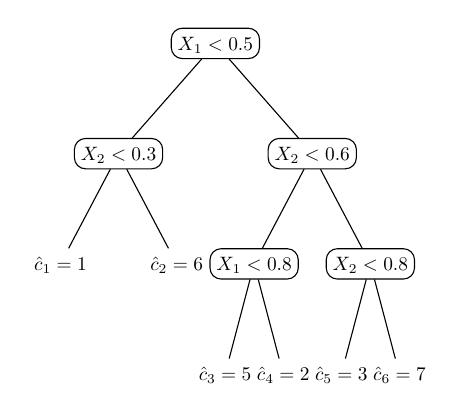
\begin{tikzpicture}[
scale = 0.7,
every node/.style={transform shape},
baseline,
level distance=20mm,
text depth=.1em,
text height=.8em,
level 1/.style={sibling distance=10em},
level 2/.style={sibling distance=6em},
level 3/.style={sibling distance=3em}]


\node [rounded corners, draw] {$X_1 < 0.5$}
child {node [rounded corners, draw] {$X_2 < 0.3$}
	child {node {$\hat{c}_1=1$}}
	child {node {$\hat{c}_2=6$}}
}
child {node [rounded corners, draw] {$X_2 < 0.6$}
	child {node [rounded corners, draw] {$X_1<0.8$}
		child {node {$\hat{c}_3=5$}}
		child {node {$\hat{c}_4=2$}}
	}
	child {node [rounded corners, draw] {$X_2<0.8$}
		child {node {$\hat{c}_5=3$}}
		child {node {$\hat{c}_6=7$}}
	}
};

\end{tikzpicture}
		\subcaption{Regression Tree based on initial data set.}
	\end{minipage}%
	\hfill%
	\begin{minipage}[c]{.45\linewidth}
		\centering
		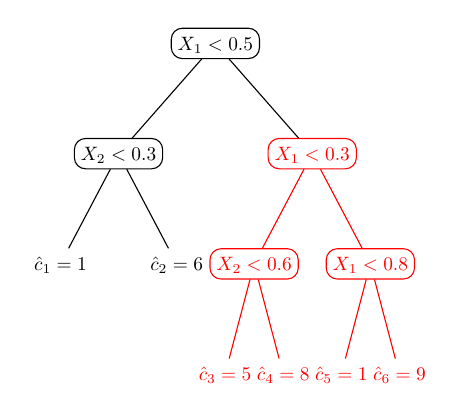
\begin{tikzpicture}[
scale = 0.7,
every node/.style={transform shape},
baseline,
level distance=20mm,
text depth=.1em,
text height=.8em,
level 1/.style={sibling distance=10em},
level 2/.style={sibling distance=6em},
level 3/.style={sibling distance=3em}]


\node [rounded corners, draw] {$X_1 < 0.5$}
child {node [rounded corners, draw] {$X_2 < 0.3$}
	child {node {$\hat{c}_1=1$}}
	child {node {$\hat{c}_2=6$}}
}
child {node [red, rounded corners, draw] {$X_1 < 0.3$}
	child [red] {node [rounded corners, draw] {$X_2<0.6$}
		child {node {$\hat{c}_3=5$}}
		child {node {$\hat{c}_4=8$}}
	}
	child [red] {node [rounded corners, draw] {$X_1<0.8$}
		child {node {$\hat{c}_5=1$}}
		child {node {$\hat{c}_6=9$}}
	}
};

\end{tikzpicture}
		\subcaption{Regression Tree based on perturbed data set.}
	\end{minipage}
	\caption[Illustration of the instability of Regression Trees.]{Illustration of the instability of Regression Trees.}
	\label{fig:Tree_Instability}
	
\end{figure}




\noindent
Figure \ref{fig:Tree_Instability} undermines the intuition behind the instability of Regression Trees with a graphical illustration. The Regression Tree in Figure \ref{fig:Tree_Instability} (a) is constructed on the basis of an initial data set. Now consider a perturbation of the data set, which leads to a different choice of splitting variable in the second layer (right node). This change affects all nodes following the altered decision rule as well (see Figure \ref{fig:Tree_Instability} (b)). Changes are indicated by red.





%Bagging
\subsection{The Implementation of Figure \ref{plot_asy}}\label{sec:App_FiniteSample}
In order to implement Figure \ref{plot_asy} from Section \ref{introductionbagging} we proceed as follows. \\
Let $Y_i \sim \mathcal{N}(0,4)$. Fix a sample $n$ from the set $\{100, 1000, 10000, 50000\}$ and denote a data set as $\mathbf{Y}=\{Y_i\}_{i=1}^n$.
The number of gridpoints for $x$ in the interval $[-5,5]$ is chosen to be $100$.
For the Bagging predictor the number of bootstrap samples is set to $B=100$.
The number of Monte Carlo iterations in order to calculate the mean squared error is also set to 100.
In every iteration step $j \in B$ at each gridpoint, we do the following:
\begin{itemize}
\item Draw a data set $\mathbf{Y_j}=\{Y_i\}_{i=1}^n$
\item Draw 100 bootstrap samples with replacement from $\mathbf{Y_j}$ and calculate for each bootstrap sample the arithmetic mean, $\bar{Y}_{n}^{*}.$
\item Calculate the bagged predictor according to Definition \ref{bagging}, that is $\hat{\theta}_{n;B}(x) = \frac{1}{100}\sum_{b=1}^{100}\mathbbm{1}_{[\bar{Y}_{n,b}^{*} \leq x]}.$
\item Calculate the squared error for the unbagged and the bagged predictor compared to $\theta(x)=\mathbbm{1}_{[0 \leq x]}$, that is $(\hat{\theta}_{n}(x)-\theta(x))^2$ and $(\hat{\theta}_{n;B}(x)-\theta(x))^2$, respectively.
\end{itemize}
Averaging over the respective squared errors gives the mean squared errors from the figure at one particular gridpoint.


\subsection{Illustration of the Bagging Algorithm applied to Regression Trees.}
\label{App:Ill_Bag}
Figure \ref{fig:Ill_Bag} illustrates the prediction procedure of the Bagging algorithm applied to Regression Trees. In this graphic $x$ is the covariate vector of new realizations.
Each Tree corresponds to a bootstrapped predictor $\hat{\theta}_n(\mathbf{x})$.
The orange paths in the trees correspond to the prediction procedure as described in Section \ref{sec:Tree_Pred}.\\
Here, + denotes the averaging over all predictions obtained by the bootstrapped predictors. The bagged prediction is denoted as $y$.

\begin{figure}[H]
\centering
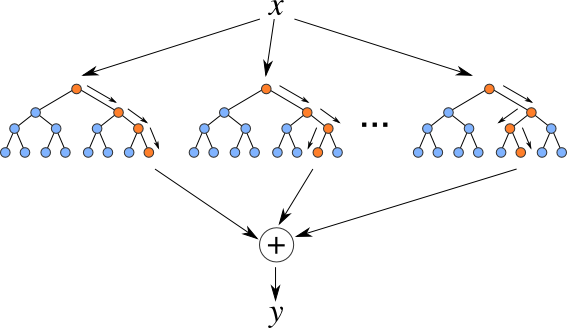
\includegraphics[scale=0.6]{external_figures/baggedtree.png}
\caption[Graphical Illustration of the Bagging algorithm applied to Regression Trees.]{Graphical Illustration of the Bagging Algorithm applied to Regression Trees. \textit{Source:} \url{http://jason-zhuo.github.io/random-forest-clustering/}.}\label{fig:Ill_Bag}
\end{figure}



%Simulation
\subsection{The Implementation of the Bagging Algorithm}\label{sec:Sim_Impl_App}
According to Definition \ref{bagging}, the Bagging Algorithm as described by \cite{Breiman1996} has been implemented in \texttt{Python} using \texttt{NumPy}. Our algorithm uses Regression Trees that are \hfill built \hfill by \hfill the \hfill \texttt{sklearn} \hfill package \hfill by \hfill \cite{scikit-learn2011}. \hfill Specifically, \hfill we \hfill use \hfill the \hfill module

\texttt{sklearn.trees.DecisionTreeRegressor}, which is a version of CART.\footnote{For further information we refer you to \url{http://scikit-learn.org/stable/modules/tree.html\#tree-algorithms-id3-c4-5-c5-0-and-cart }.} Building the optimal Regression Tree is computationally infeasible as shown by \cite{Hyafil1976}. To bypass this problem partially, \texttt{sklearn} uses a slightly optimized version of the CART-Algorithm.\footnote{\texttt{Sklearn} selects a single Regression Tree by training multiple Trees, where the features and corresponding observations are randomly sampled with replacement. Note that this random selection procedure was not used in the original CART-Algorithm introduced by \cite{Breiman1984}. The \texttt{sklearn} algorithm stays close to CART in the other aspects and is therefore a reasonable choice for the simulation studies. See \url{http://scikit-learn.org/stable/modules/tree.html\#decision-trees} for further information on this.}

The Bagging algorithm itself can be described as follows:\footnote{This pseudo code was inspired by \url{http://pages.cs.wisc.edu/~matthewb/pages/notes/pdf/ensembles/RandomForests.pdf}.}

\begin{algorithm}
    \caption{Bagging Algorithm with Regression Trees}
    \label{fit-bagging}
    \begin{algorithmic}[1] % The number tells where the line numbering should start
      \Require Training Sample $L = \{y_{i},\mathbf{x_{i}} \}_{i=1}^{n}$ and $B$ number of bootstrap iterations

        \Function{BaggingAlgorithm}{$L,B$}
            \State{$T \gets  \emptyset$} \Comment{T is the container for all following Trees}
            \For{$j$ in 1 to $B$}
                \State $L^{j*} \gets $ Draw bootstrap sample from $L$
                \State $t^j \gets$ \Call{RegressionTree}{$L^{j*}$}
                \State $T \gets T \cup t^j$
            \EndFor
            \State \textbf{return} $T$
        \EndFunction

        \Function{RegressionTree}{$L^*$}
        \State $t \gets$ Train Regression Tree on $L^*$
        \State \textbf{return} $t$
        \EndFunction
    \end{algorithmic}
\end{algorithm}

Once we have applied the Bagging Algorithm with Regression Trees to some training set $L$, we can make a prediction on a test set $G$ in the following way:

\begin{algorithm}
  \caption{Prediction for Bagging Algorithm with Trees}
  \label{predict-bagging}
  \begin{algorithmic}[1] % The number tells where the line numbering should start
    \Require Test Sample $G = \{y_{i},\mathbf{x_{i}} \}_{i=1}^{m}$ and a trained Bagging instance $T$ as defined by Algorithm \ref{fit-bagging} consisting of $B$ different Regression Trees
    \Function{PredictBagging}{$G,T$}
      \For{$j$ in 1 to $B$}
      \State $p^j \gets$ Prediction with $t^j \in T$ for $G$
      \State $P \gets P \cup p^j$
      \EndFor
      \State $A \gets$ For each observation $j \in G$ average over all $B$ predictions in $P$
      \State \textbf{return} $A$
    \EndFunction

  \end{algorithmic}
\end{algorithm}

The array $A$ then consists of the averaged predictions, based on the trained Bagging instance $T$, for each observation in the training set $G$ and is therefore of shape $(m,1)$. Hence, we make for each observation in the training set $G$, $B$-many predictions and average over those outcomes to obtain the array of final predictions.

\begin{comment}
\subsection{Tree Depth and Bagging}\label{sec:Sim_TreeDepth}
In the simulation employed in Section \ref{sec:Simulation}, we always choose to grow the Trees fully. In this part we want to give some insight why this is optimal, when Bagging is applied to Regression Trees. \newline
As discussed in Section \ref{sec:BiasVariance}, Regression Trees tend to overfit the data. Overfitting is specifically a problem, when we grow a Tree to its maximal size. The terminal leafs will consist of only a single observation, making it thereby likely that we fit the noise in the data. Thus usually when fitting single Trees to the data it is common to restrict the size of the Tree to reduce overfitting and thereby reduce the variance. \newline
Interestingly, it turns out that it is \textit{not} the optimal choice in terms of MSPE to restrict the Tree size if we apply Bagging to Regression Trees as we can see in Figure \ref{fig:leafsize}.
\begin{figure}[H]
\centering

\includegraphics[scale=0.6]{../../out/figures/main_simulation/plot_simulation_tree_depth.pdf}
\caption[The effect of varying the complexity of the Regression Tree for the normal and bagged Tree.]{The effect of varying the complexity of the Regression Tree for the normal and bagged Tree. The minimal size for each leaf is displayed on the $x$-axis. A higher minimal size for each leaf implies a less complex Tree.}
\label{fig:leafsize}
\end{figure}

In Figure \ref{fig:leafsize} we plot the MSPE, the variance and the squared-bias for bagged and unbagged Trees against the Tree depth. We control the size of each Tree by restricting the minimal amount of observations in each terminal node. A larger minimal size for each terminal node implies a smaller and thus less complex Tree.
We report the results for the unbagged Regression Tree and Bagging applied to Regression Trees as in Section \ref{sub:bagging_table} for both regression functions.
\newline
The MSPE for Trees is minimized at a smaller Tree size as for Bagging. Whereas for Bagging we obtain the best result by growing the Tree to the maximal length, the optimum for normal Regression Trees can be achieved by restricting the minimal size for each terminal node to around 20 observations. Lower values result in a higher MSPE for Trees. While we decrease the squared-bias by increasing the size of the Tree, we overfit the data and have a predictor with a high variance. \newline
Bagging on the other hand works best if there are no restrictions on the Tree size. As discussed in Section \ref{bag} and \ref{sec:bagregtree}, Bagging reduces the variance of the predictor while leaving the squared-bias almost unaffected. As Regression Trees have the lowest bias for maximal grown Trees, it is therefore optimal not to restrict the size of the Trees, when using Bagging.
\end{comment}


%Real Data
%\subsection{Real Data Application: List of variables}
%\label{sec:VariableList}

%Endogenous:
%\begin{enumerate}
%\item housing values
%\begin{itemize}
%\item median value of homes in thousands of dollars
%\end{itemize}
%\end{enumerate}

%Explanatory:
%\begin{enumerate}
%\item socio-economic
%	\begin{itemize}
%	\item crime rate
%    \item tax-rate
%    \item pupil/teacher ratio
%    \item percentage black
%    \item percentage lower-status population
%	\end{itemize}
%\item geographical-economic
%	\begin{itemize}
%	\item percentage land zoned for lots
%    \item percentage nonretail business
%    \item river dummy (1 if on Charles River, 0 otherwise)
%    \item weighted distance to employment centers
%    \item accessibility to radial highways
%	\end{itemize}
%\item property characteristics
%	\begin{itemize}
%    \item average number of rooms
%    \item percent built before 1940
%    \end{itemize}
%\item Pollution
%	\begin{itemize}
%	\item nitrogen oxide concentration, pphm
%	\end{itemize}
%\end{enumerate}

%For a detailed variable description see \citet[p.96-97]{Harrison1978}.















\end{appendix}

\newpage

\setstretch{1}
\printbibliography
\setstretch{1.5}


%\bibliographystyle{agsm}
%\bibliography{Bibliography/MetricsBibliography.bib}



\end{document}

